\section{Безопасность в статистических БД}

Инфы про статистические базы данных на русском языке мало и большая часть бредовая. Гуглите statistical database. Все источники будут на английском, переведено специально для вас. Источников несколько \cite{ComputerSecurity2008} \cite{IntroBD2014}, под конец была найдена статья, \cite{SDB1989} в которой есть вся собранная инфа.

\subsection{Общие сведения}.
Определение статистической БД. Классификация статистических БД. Характеристики статистических БД.

Статистической (в приведенном здесь контексте) называется база данных, в которой допускаются запросы с обобщением данных (суммированием, вычислением среднего значения и т.д.), но не допускаются запросы по отношению к элементарным данным. Например, в статистической базе данных разрешается выдача запроса "Какова средняя зарплата программистов?", тогда как выдача запроса "Какова зарплата программиста Мэри?" запрещена.
Проблема статистических баз данных заключается в том, что иногда с помощью логических заключений на основе выполнения разрешенных запросов можно вывести ответ, который прямо может быть получен только с помощью запрещенного запроса. "Обобщенные значения содержат следы исходной информации, и она может быть восстановлена злоумышленником после соответствующей обработки этих обобщенных значений. Такой процесс называется логическим выводом конфиденциальной информации".
Практически для любой статистической базы данных всегда может быть определен общий трекер (в отличие от множества индивидуальных трекеров). Общий трекер (general tracker) — это логическое выражение, которое может быть использовано для поиска ответа на любой запрещенный запрос, т.е. запрос, включающий недопустимое логическое выражение. (В противоположность этому индивидуальный трекер работает только на основе запросов, включающих конкретные запрещенные выражения.)
Требуется поддерживать баланс между репрезентативностью данных и конфиденциальностью отдельных записей.

\subsection{Классификация}
Классифицирует по следующим признакам:
\begin{itemize}

    \item Чисто статистическая база данных - Обычная база данных со статистическим доступом

этот тип базы данных хранит только статистические данные. Примером может служить база данных переписи населения.
этот тип базы данных содержит отдельные записи. Кроме того, база данных поддерживает набор статистических пользователей, которым разрешены только статистические запросы. Для этих последних пользователей совокупная статистика, основанная на базовых необработанных данных, генерируется в ответ на запрос пользователя или может быть предварительно вычислена и сохранена как часть базы данных.

    \item Оффлайн-Онлайн

В онлайн-SDB существует прямое взаимодействие пользователя с данными в режиме реального времени через терминал. В автономном SDB пользователь не контролирует обработку данных и не знает, когда выполняется его запрос данных. В этом режиме методы защиты, отслеживающие профили пользователей, становятся более громоздкими. Компромиссные методы, требующие большого количества запросов (например, метод компромисса на основе регрессии, см. Раздел 7), также усложняются при работе в автономном режиме.

    \item Статическая-Динамический

Статическая база данных-это такая база данных, которая никогда не меняется после ее создания. Большинство баз данных переписи являются статическими. Всякий раз, когда создается новая версия базы данных, эта новая версия считается другой статической базой данных. В отличие от этого, динамические базы данных могут изменяться непрерывно. Эта особенность может значительно усложнить проблему безопасности, поскольку частые выпуски новых версий могут позволить ищейкам использовать различия между версиями способами, которые трудно предвидеть. Методы возмущения данных могут не подходить для динамических СДБ, так как усилия по преобразованию исходного СДБ в возмущенный могут стать непомерными.

    \item Централизованный-Децентрализованный

В централизованном SDB есть одна база данных. В децентрализованном (распределенном) SDB перегруженные подмножества базы данных хранятся на различных узлах, Соединенных коммуникационной сетью. Распределенная база данных может быть полностью реплицирована, частично реплицирована или секционирована. Проблема безопасности распределенного SDB является более сложной, чем проблема централизованного SDB из-за необходимости дублировать на каждом узле накладные расходы по контролю безопасности, а также трудности интеграции профилей пользователей.
Выделенная-общая компьютерная система в выделенной SDB компьютерной системе используется исключительно для обслуживания приложений SDB. В общей системе приложения SDB работают на одной аппаратной системе с другими приложениями (возможно, с использованием различных баз данных). Общую среду защитить сложнее, так как другие приложения могут вмешиваться в защищаемые данные непосредственно через операционную систему, минуя механизм безопасности SDB.
\end{itemize}
\subsection{Угрозы статистических БД}

Об безопасности в статистических БД  Деннинг [16.6]
\begin{grayquote}
"методы нарушения защиты данных просты и не связаны с большими расходами. Поэтому требование обеспечения полной секретности конфиденциальной информации несовместимо с требованием возможности вычисления точных статистических показателей для произвольных подмножеств данных в базе. По крайней мере одно из этих требований должно быть снято прежде, чем можно будет поверить в гарантии обеспечения секретности.
\end{grayquote}
То есть существует мнение, что нельзя нормально обезопасить СБД.

Основная проблема СБД -- проблема вывода.
В общих чертах, проблема вывода для SDB может быть сформулирована следующим образом. Характеристическая функция C определяет подмножество записей (строк) в базе данных. Запрос, использующий C, предоставляет статистику по выбранному подмножеству. Если подмножество достаточно мало, возможно, даже одна запись, спрашивающий может быть в состоянии сделать вывод о характеристиках одного человека или небольшой группы. Даже для больших подмножеств характер или структура данных могут быть такими, что несанкционированная информация может быть выпущена.
Для злоумышленика, который пытается достать индивидуальные данные задача состоит в том, чтобы сделать общий трекер.
Нужно придумать такую последовательность запросов, чтобы вывести индививидуальную информацию.
Суть в том, что можно набрать несколько запросов и проделать операции над ними там, чтобы деанонить записи.

Например для статичной СБД можно сделать такое

запрос1: выдать a1 + a2 + a3, запрос2: выдать a1 + a2. запрос1 - запрос2 = a3.

Для динамической онлайн СБД
Мы хотим достать зарплату Мэри. Знаем, что ей 20 лет. Записываем в базу много левых записей с возрастом = 20 лет и нулевой зарплатой. Делаем запрос с минимальной агрегацией людей с возврастом 20 лет. Таким образом можно узнать возможную зп Мэри. Чем больше исходных знаний есть о Мэри, тем точнее получим данные.
Также не стоит забывать что речь идет о БД. Поэтому статистическая БД наследует все опасности обычных БД.

  \subsection{Защита в статистических БД}

Разделяют четыре общих подхода защиты статистических БД:
\begin{itemize}
  \item концептуальный;
	\item ограничение запросов;
	\item возмущение данных;
	\item возмущение вывода;
\end{itemize}
На рисунке \ref{fig:SDB_secure} изображена схема 3 подходов.
\begin{figure}[h]
    \centering
    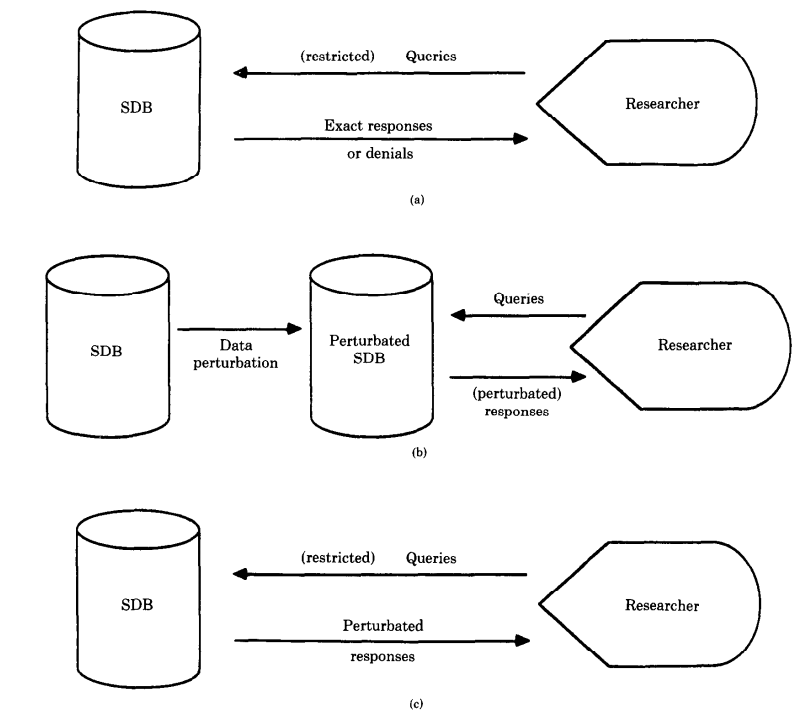
\includegraphics[width=0.8\textwidth]{assets/SDB_secure_method.png}
    \caption{Схемы безопасности СДБ}
    \label{fig:SDB_secure}
\end{figure}
\paragraph{Концептуальный}

Основная проблема в том, что вся реляционная алгебра позволяет выводить индивидуальные данные. Концептуальный подход предлагает заменить классическую систему реляционной БД работающую с индивидуальными данными.
Основной подход:
Partitioning of the data base -- Записи хранятся не отдельно, а агрегировано и обезличино. Судя по-всему похоже на microagregation.
Microaggregation -- есть исходные данные, выделим несколько записей, посчитаем для них средние значения, заменим значения записей полученным средним, повторить для остальных записей в исходных данных

Еще один способ -- решетчатая модель. Агрегация данных по разным признакам на разном уровне детализации.

Ну и естественно не забываем про классические способы.
Access Restriction - пусть вы доктор, тогда вам можно всё. А исследователям и прочим анонам даём только некоторые записи или даже готовые стат.результаты по данным (агрегация)

\paragraph{Ограничение запросов}

Query Set Restriction -- Ограничение на минимальный размер выдаваемой выборки.

Limiting intersection of query sets --  Метод защиты блокирует такие запросы которые приводят к выводу данных через пересечение множеств запросов.
Сохранение исторических сведений о результатах выполнения запросов и отклонение любых запросов, использующих значительное количество исходных данных, обработанных предыдущим запросом.
Auditing - ведём логи, ловим негодяев и всяких подознительных

\paragraph{Возмущение данных}

Data Perturbation -- добавим небольшой, случайный шум. Тогда точные данные вроде как и будут уничтожены, но можно заиграться и исказить репрезентативность

Случайное добавление дополнительных строк к основному набору данных, обрабатываемому запросом.
Также предлагается организовать "обмен данными" ("data swapping"), т.е. обмен значениями атрибутов между кортежами, осуществляемый таким образом, чтобы поддерживалась лишь статистическая точность. При этом даже если злоумышленнику удастся идентифицировать отдельное значение (например, некоторое значение зарплаты), то у него не будет способа узнать, какому именно кортежу (в нашем примере — сотруднику) оно принадлежит. Сложность этого подхода заключается в необходимости отыскать множество тех записей, между которыми можно будет организовать обмен значениями соответствующим образом. Подобные затруднения имеют место и при использовании большинства других методов.

\paragraph{Возмущение вывода}

Output Perturbation -- как предыдущее, но преобразовывать будем результат каждого запроса
Random Sampling -- сделать так, чтобы один и тот же запрос давал каждый раз разные наборы записей
Использование для ответов на запросы только случайных наборов исходных данных

\paragraph{Критерии безопасности}
Как было сказано гарантированной безопасности в СДБ не добиться. Поэтому делают оценку важности деанонимизированных данных и статистической точности (из-за наших всех действий для защиты данных)

Security -- сферическая вероятность раскрыть (в том числе частично) запись в сбд
Для каждого разрешенного агрегирующего запроса оценивается критерий безопасности. На основе количества инфы в базе можно подсчитать сколько тех или иных запросов нужно сделать для деанонимизации. На основе этого расчитывается минимальная выборка для таких запросов.

Consistency -- оценивается консистентность данных для методов возмущения данных. Оценивается степень возмущения данных. Создаем агрегирующий запрос и замеряем его изменения после внесенных возмущений.
Robustness -- оценка зависимости между возмущением и конкретной записью. Было бы круто чтобы возмущение не было зависимо от данных, но нужно каким-то образом сохранить ее статистические свойства.

Costs -- Назначаем каждому запросу конкретную цену. Пользователю даем начальную сумму на которую он может делать запросы, такую чтобы он не смог вывести данные. Выглядит больше как метод, а не критерий.
